% This is an example document accompanying "LaTeX for Administrative Work"
% See www.dickimaw-books.com/latex/admin/ for the book details,
% including licence.

% Arara directives to build the document:
%
% arara: pdflatex
% arara: pdflatex

\documentclass{beamer}
%\useinnertheme{circles}
\usetheme{Boadilla}
\newcommand{\myitem}{\item[\textbullet]}


\AtBeginSection[]{
  \begin{frame}
  \vfill
  \centering
  \begin{beamercolorbox}[sep=8pt,center,shadow=true,rounded=true]{title}
    \usebeamerfont{title}\insertsectionhead\par%
  \end{beamercolorbox}
  \vfill
  \end{frame}
}
\usepackage[T1]{fontenc}
\usepackage[utf8]{inputenc}
\usepackage{multirow}

\title{Dating Problem via Linear Programming}
\author{}
\date{}
%\institute{\inst{1}Institute of Computing Technology,\\Chinese Academy of Sciences\\
%
%  \inst{2}Department of Computer Science,\\City University of Hong Kong\\
%  \inst{3}Shenzhen Institutes of Advanced Technology, \\Chinese Academy of Sciences\\
%}
%\titlegraphic{\includegraphics[width=1in]{dummy-logo}}

\begin{document}
\beamerdefaultoverlayspecification{<+->}
\begin{frame}
  \maketitle
\end{frame}
\setbeamertemplate{section in toc}[circle]
\setbeamertemplate{subsection in toc}[square]
\setbeamertemplate{itemize items}[circle]
\begin{frame}{Overview}\centering
\tableofcontents
\end{frame}
\section{Problem Description}

\begin{frame}
  \frametitle{Problem Description}
  \begin{block}{Classical Dating Problem (Secretary Problem)}
  \begin{itemize}
	\item \textbf{Suppose} you are going to dating with several boys/girls one by one
	\item These persons come in a uniform random order
	\item As you are a decent person, you will make decision immediately after dating with each boys/girls:
  	\begin{itemize}
	  \item If current person is chosen, you will not dating with
			 unseen ones;
	  \item If current one is rejected, you can continue dating with
			 next one, however, the rejected one will never come back.
   \end{itemize}
  \item Certainly, you want to select the best boy/girl as your soul mate
  \item So, how to design a strategy to maximum the probability that the best
		  one is chosen?
  \end{itemize}
  \end{block}
\end{frame}

\begin{frame}
	\frametitle{Example}
	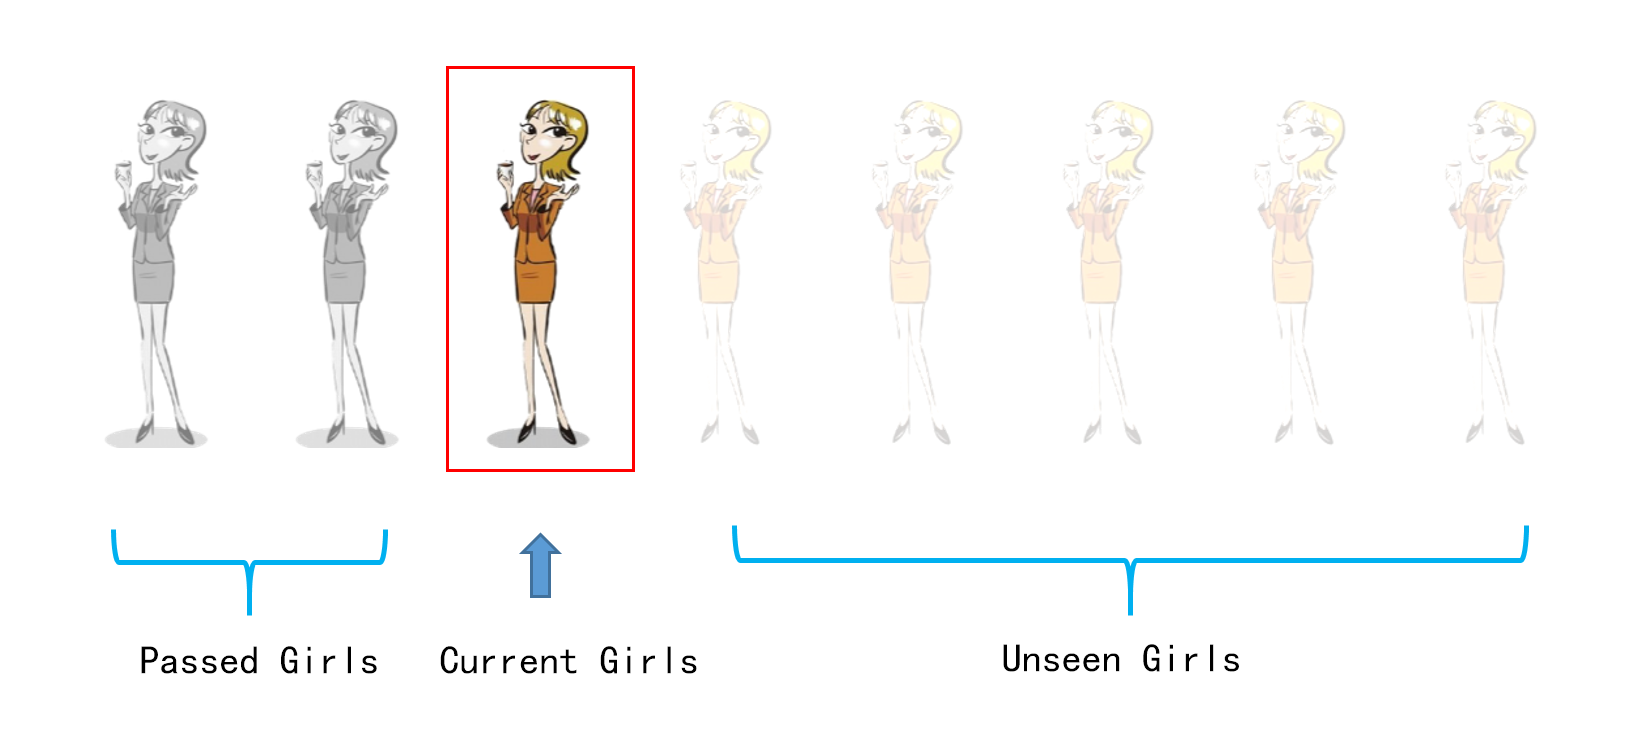
\includegraphics[width=12cm]{Problems/secretary1.png}
\end{frame}

\begin{frame}{Problem Analysis}
		\begin{block}{Hardness of Dating Problem}
  \begin{itemize}
  \item Lack of information: when you make decision for current person, you have no information about future ones
  \item One-shot decision: Once you make a decision on a person, you have no chance to regret
  \end{itemize}
  \end{block}
\end{frame}

\section{Linear Programming Model}

\begin{frame}{Linear Programming Model}{Analysis}
%\begin{block}{Analysis}
\begin{itemize}
  \item Suppose there are $n$ persons to date with
  \item In any \emph{reasonable} algorithm, if you want to select a person as your soul mate, she/he must be the best one up to now
  \item Let $x_i$ stand for the probability that the $i$-th one is chosen given she/he is the best person from position 1 to $i$ 
  \item That's to say
		  \begin{equation}
				  \begin{split}
				  x_i &= \Pr[\text{The $i$-th one is selected}\\
				  &\qquad\quad|\text{The $i$-th one is the best one from 1 to $i$}]
				  \end{split}
		  \end{equation}
\end{itemize}
\begin{block}{Remark}
		  It should be emphasis that the probability $x_i$ is defined on the randomness of coming sequence
\end{block}
%\end{block}
\end{frame}

\begin{frame}{Linear Programming Model}{Analysis}
%\begin{block}{Analysis}
\begin{itemize}
  \item Clearly, we have 
		  \begin{equation*}
				  \begin{split}
						  x_i &\leq \Pr[\text{No one is selected before position $i$}]\\
						  %&1-\Pr[\text{One person on position 1 to $i-1$ is selected}]\\
						  &=1-\sum_{l = 1}^{i-1}\Pr[\text{The $l$-th one is selected}]\\
						  &=1-\sum_{l = 1}^{i-1}\frac{1}{l}\cdot x_l
				  \end{split}
		  \end{equation*}
\end{itemize}
%\end{block}
\end{frame}

\begin{frame}{Linear Programming Model}{Analysis}
\begin{itemize}
\item Let $Z$ stand for the event that the best person is chosen
\item It is clearly that
		\begin{equation}
				\begin{split}
						\Pr[Z] &= \sum_{i = 1}^n \Pr[\text{The $i$-th one is the best person and she/he is chosen}]\\
						&= \sum_{i=1}^n\Pr[\text{The $i$-th one is the best person}]\\
						&\qquad\cdot\Pr[\text{The $i$-th one is selected}|\text{The $i$-th one is the best person}]\\
						&= \sum_{i=1}^n\frac{1}{n}\cdot x_i
				\end{split}
		\end{equation}
\end{itemize}
\end{frame}

\begin{frame}{Linear Programming Model}{Primal}
\begin{itemize}
\item In summary we have the following LP model:
		\begin{equation}
				\begin{split}
						&\text{\bf Maximize: } \Pr[Z] = \sum_{i=1}^n x_i\\
						&\begin{aligned}
								&\text{\bf s.t.}& & x_i \leq 1-\sum_{l = 1}^{i-1}\frac{1}{l}\cdot x_l, & &1\leq i \leq n&\\
								& & &x_i \geq 0, & &1\leq i \leq n.&
						\end{aligned}
				\end{split}
		\end{equation}
\item So simple a LP model!
\end{itemize}
\end{frame}

\begin{frame}{Linear Programming Model}{Dual}
\begin{itemize}
  \item Recall the relationship between the primal LP and its dual 
  \item Let $y_i$ stand for the dual variable of $x_i$
  \item We have the following dual LP of the Dating Problem:  
		\begin{equation}
				\begin{split}
						&\text{\bf Minimize: } \sum_{i=1}^n y_i\\
						&\begin{aligned}
								&\text{\bf s.t.}& & y_i +\frac{1}{i}\sum_{l = i+1}^{n} y_l\geq \frac{1}{n}, & &1\leq i \leq n&\\
								& & &y_i \geq 0, & &1\leq i \leq n.&
						\end{aligned}
				\end{split}
		\end{equation}
  \item What's the meaning of $y_i$? 
  \item It is an open problem. Clever as you may have some idea. 
\end{itemize}
%\begin{example}\end{example}
\end{frame}
%\section{Background}

\begin{frame}{Linear Programming Model}{Strictness of the LP Model}
\begin{itemize}
    \item Although simple, the primal LP \emph{strictness} for Dating Problem
	\item \emph{Strictness} means any algorithm can be mapped to a feasible solution of the LP and any solution of the LP can be mapped to an algorithm
	\item Why strictness is important?
	\item Only when a LP is strict, the optimal solution of the LP can be an optimal solution for the problem
\end{itemize}
\end{frame}

\begin{frame}{Linear Programming Model}{Strictness of the LP Model}
\begin{itemize}
	\item It easy to check that any algorithm $\pi$ can be mapped to a feasible solution of the primal LP:
	\begin{itemize}
				\item We can calculate the value $x_i$ in $\pi$ 
				\item Then, we can check that these $x_i$s obtained satisfies the constraint 
				\item We omit this proof here. (Maybe a homework?)
			\end{itemize}
	\item We should show that any feasible solution can be mapped to an algorithm for Dating Problem
\end{itemize}
\end{frame}

\begin{frame}{Linear Programming Model}{Strictness of the LP Model}
\begin{itemize}
		\item Suppose $\{x'_i| 1\leq i\leq n\}$ is a set of feasible solution of the primal LP
		\item We construct an algorithm $\pi$ based on $x'_i$ as follow:
			\begin{itemize}
			\item For each person $j$, if she/he is the best one up to now, select is with probability $\frac{x_i}{1-\sum_{l = 1}^{i-1}\frac{1}{l}\cdot x_l}$
		    \item Otherwise, that's $j$ is not the best one up to now, discard she/him
			\end{itemize}
	\item It's over?
	\item Naive! We should show that $x_i(\pi) = x'_i$, where $x_i(\pi)$ is the probability that $i$-th one is selected give she/he is the best one up to $i$ in algorithm $\pi$
	\item Think about why we should show this and show it by yourself (May a homework?)
\end{itemize}
\end{frame}
\section{Optimal Algorithm}
\begin{frame}{Optimal Algorithm}{Randomized}
	\begin{itemize}
		\item Somehow we have solved the Dating Problem:
			\begin{itemize}
				\item Solve the primal LP
				\item Construct an algorithm based on the optimal solution of LP as previous slides
				\item Finally, we have an optimal randomized algorithm
			\end{itemize}
	    \item It is not over so far
	\end{itemize}
\end{frame}

\begin{frame}{Optimal Algorithm}{Deterministic}
	\begin{itemize}
		\item In fact, there is an optimal deterministic algorithm for the Dating Problem:
			\begin{itemize}
					\item For the first $\frac{n}{e}$ persons, you just dating but select nobody
				\item For the rest persons, select the first one that better than all previous
			\end{itemize}
	\item By this algorithm, you can find your soul mate with probability $\frac{1}{e}$
	\end{itemize}
\end{frame}

\begin{frame}{Optimal Algorithm}{Deterministic}
	\centering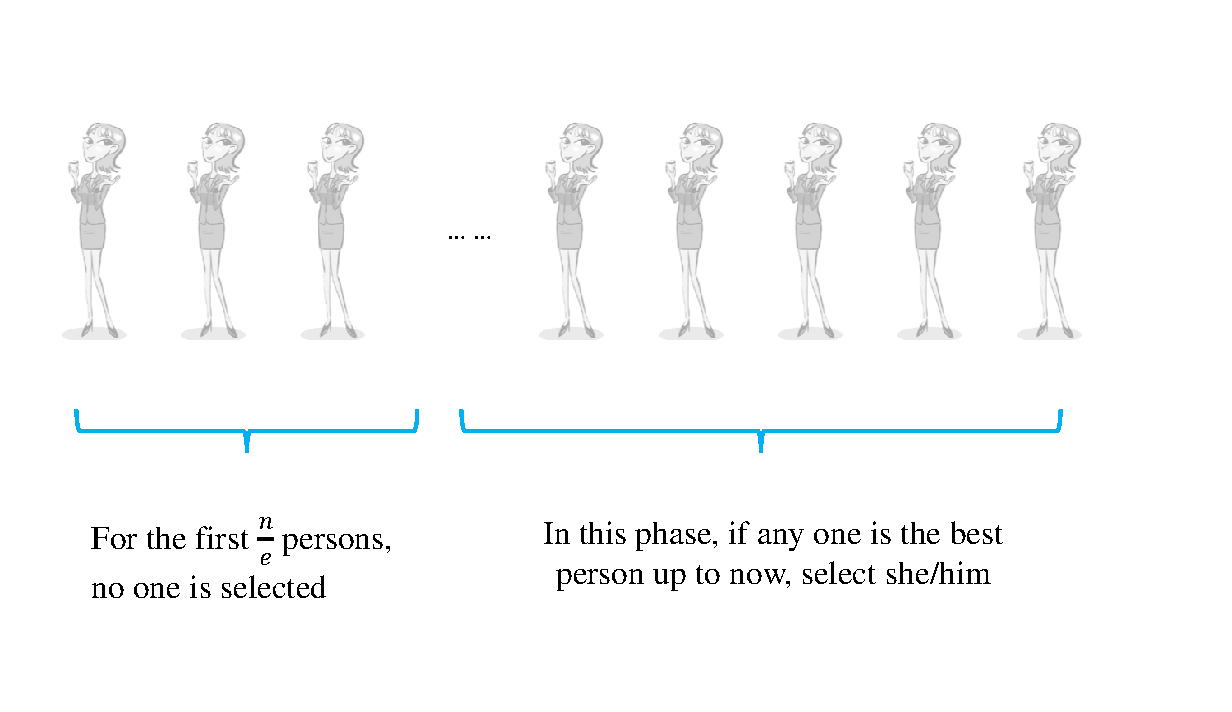
\includegraphics[width=13cm]{Problems/present-1}
\end{frame}

\begin{frame}{Optimal Algorithm}{Deterministic}
	\centering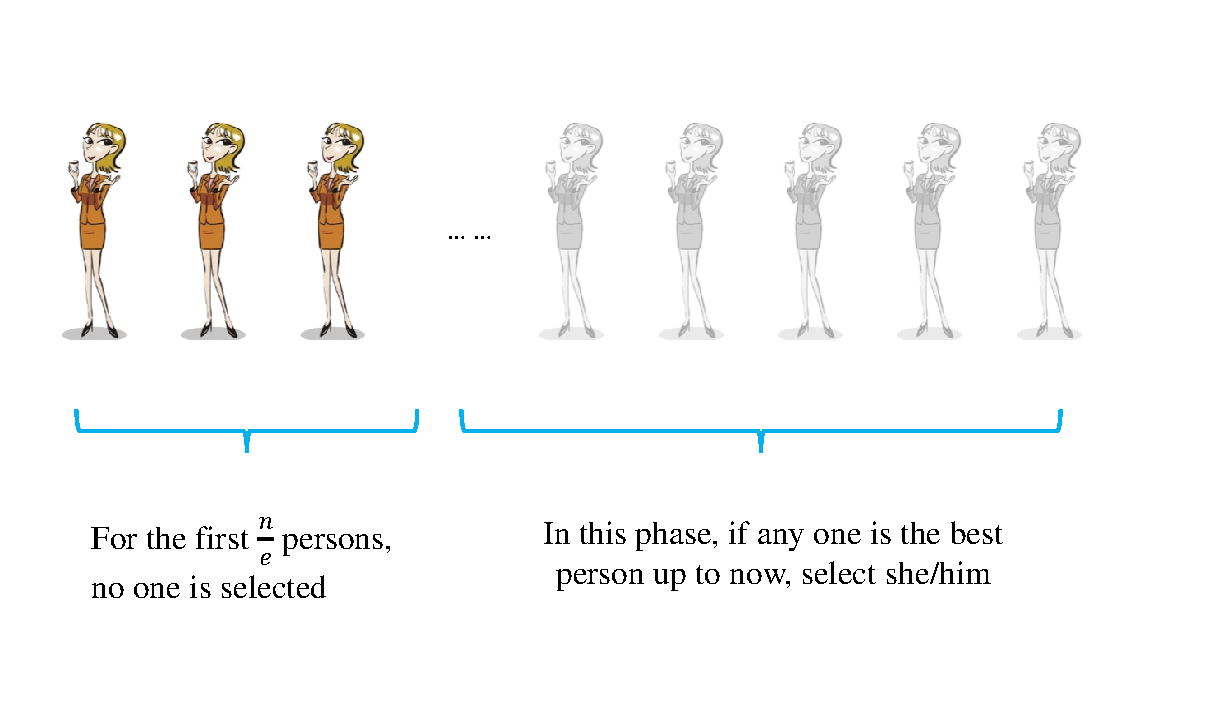
\includegraphics[width=13cm]{Problems/present-2}
\end{frame}

\begin{frame}{Optimal Algorithm}{Deterministic}
	\centering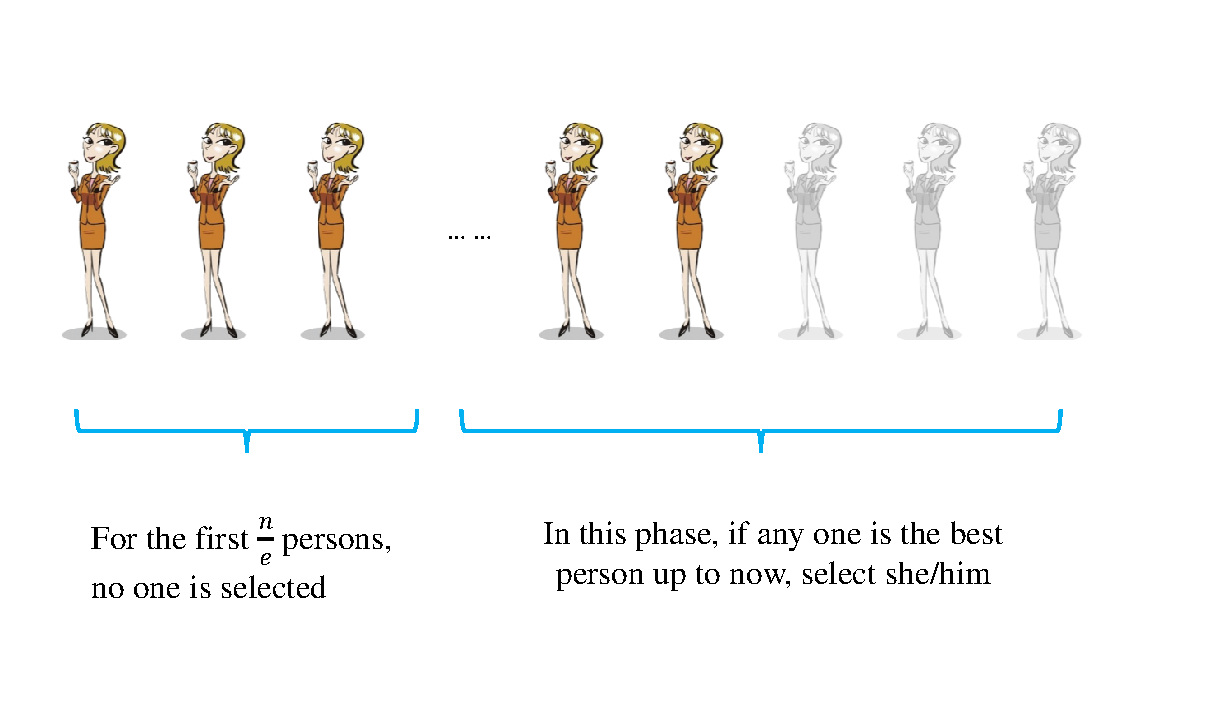
\includegraphics[width=13cm]{Problems/present-3}
\end{frame}
\begin{frame}{Optimal Algorithm}{Deterministic}
	\centering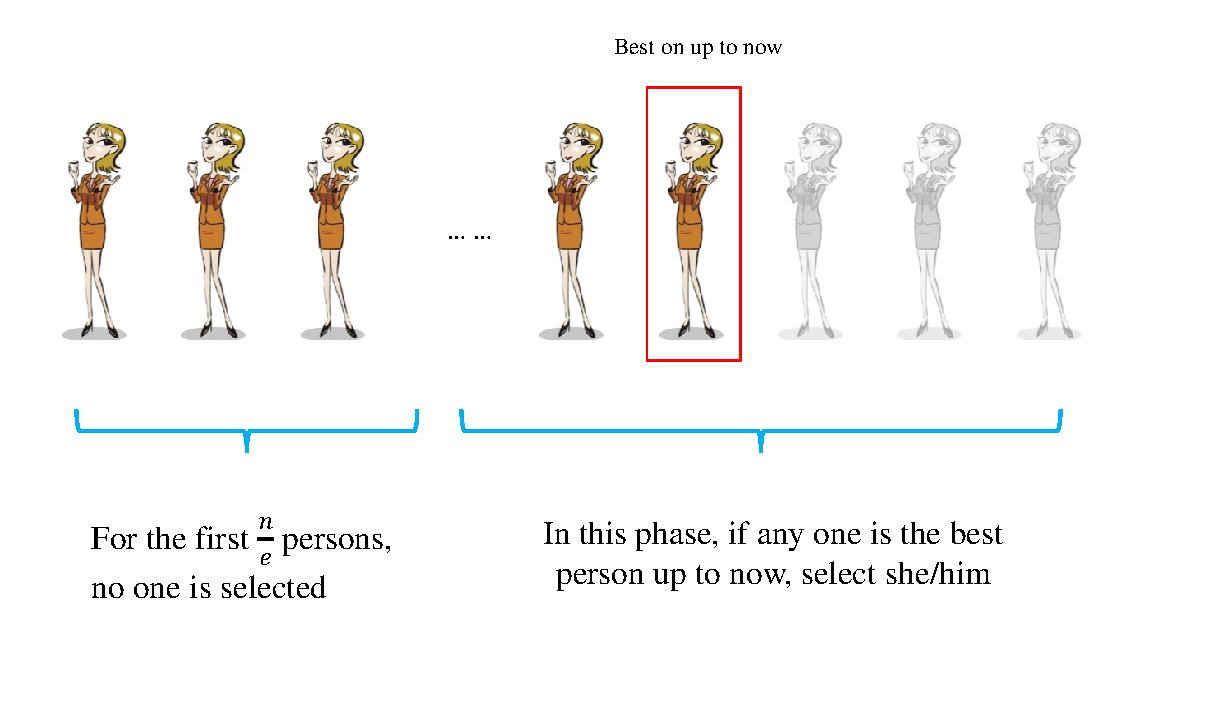
\includegraphics[width=13cm]{Problems/present-4}
\end{frame}

\begin{frame}{Optimal Algorithm}{Deterministic}
	\begin{itemize}
		\item This deterministic algorithm can be mapped to an feasible solution $\{x_i|1\leq i\leq n\}$ of the primal LP that satisfies
			\begin{itemize}
					\item $x_i = 0$, for $1\leq i\leq \frac{n}{e}$
					\item $x_i = 1-\sum_{l = 1}^{i-1}\frac{1}{l}\cdot x_l$, otherwise
			\end{itemize}
		\item This is easy to check
		\item By solve some small case using GLPK, we can find the optimal solution is exactly in this pattern
		\item How to show that for general $n$ the deterministic algorithm is optimal?
		\item We will show the optimality by the Theorem of Complementary Slackness
	\end{itemize}
\end{frame}
\begin{frame}{Optimal Algorithm}{Feasible Solution of Dual LP}
	\begin{itemize}	
		\item We first construct an feasible solution of the dual LP
		\item Fixed the constraint of the dual LP tight, that's let 
				$$y_i +\frac{1}{i}\sum_{l = i+1}^{n} y_l = \frac{1}{n}$$
		\item Solve this recursion from $n$ to $1$
		\item We can get that $y_i=\frac{1}{n}\left(1-\sum_{l = i}^{n-1}\frac{1}{l}\right)$
		\item Clearly, $y_i$ is decrease as $i$ going down
		\item When $n$ is large enough we have $y_i \approx \frac{1-log n/i}{n}$ and it equals to 0 exactly when $i = \frac{n}{e}$!
		\item According to the non-negative constraint we set $y_i$ to be 0 when $1\leq i \leq \frac{n}{e}$
	\end{itemize}
\end{frame}
\begin{frame}{Optimal Algorithm}{Feasible Solution of the Primal and Dual LP}
	\begin{itemize}
		\item In summary, we have a feasible solution of the dual LP that satisfies:
				\begin{equation}
					y_i = \left\{\begin{aligned}
							&0,& &1\leq i\leq n/e&\\
							&\frac{1}{n}-\frac{1}{i}\sum_{l = i+1}^n y_l& &n/e < i\leq n&
					\end{aligned}
					\right.
				\end{equation}
		\item The deterministic algorithm can be mapped to an feasible solution of the primal LP that satisfies:
				\begin{equation}
					x_i = \left\{\begin{aligned}
							&0,& &1\leq i\leq n/e&\\
							&1-\sum_{l = i+1}^n \frac{1}{l}x_l& &n/e < i\leq n&
					\end{aligned}
					\right.
				\end{equation}
	\end{itemize}
\end{frame}

\begin{frame}{Optimal Algorithm}{Slackness Variable of the Primal and Dual LP}
	\begin{itemize}
		\item Let $xs_i$ and $ys_i$ stand for the corresponding slackness variable of $x_i$ and $y_i$, we have 
				\begin{equation}
					xs_i  \left\{\begin{aligned}
							&\geq 0,& &1\leq i\leq n/e&\\
							&= 0& &n/e < i\leq n&
					\end{aligned}
					\right.
				\end{equation}
				\begin{equation}
					ys_i  \left\{\begin{aligned}
							&\geq 0,& &1\leq i\leq n/e&\\
							&= 0& &n/e < i\leq n&
					\end{aligned}
					\right.
				\end{equation}

			\item Easy to check that those tow feasible solutions satisfy the Theorem of Complementary Slackness 
	\end{itemize}
\end{frame}
\begin{frame}
		\centering Thanks!
\end{frame}
\end{document}

